%%%%%% CMB-S4 Simulations and Data Analysis Chapter, Component Separation Section  %%%%%%%%%%%%%%%%

\section{Component Separation}

\textbf{ Authors: Mark Ashdown, Jonathan Aumont, Carlo Baccicalupi, Josquin Errard, Maude Le Jeune}

Key challenges:
\begin{itemize}
\item validation - are we using the right algorithms for the (as yet unknown) real foregrounds
\item verification - are these algorithms right given our (as yet flawed) simulations
\end{itemize}

\begin{figure*}[htbp]
\centering
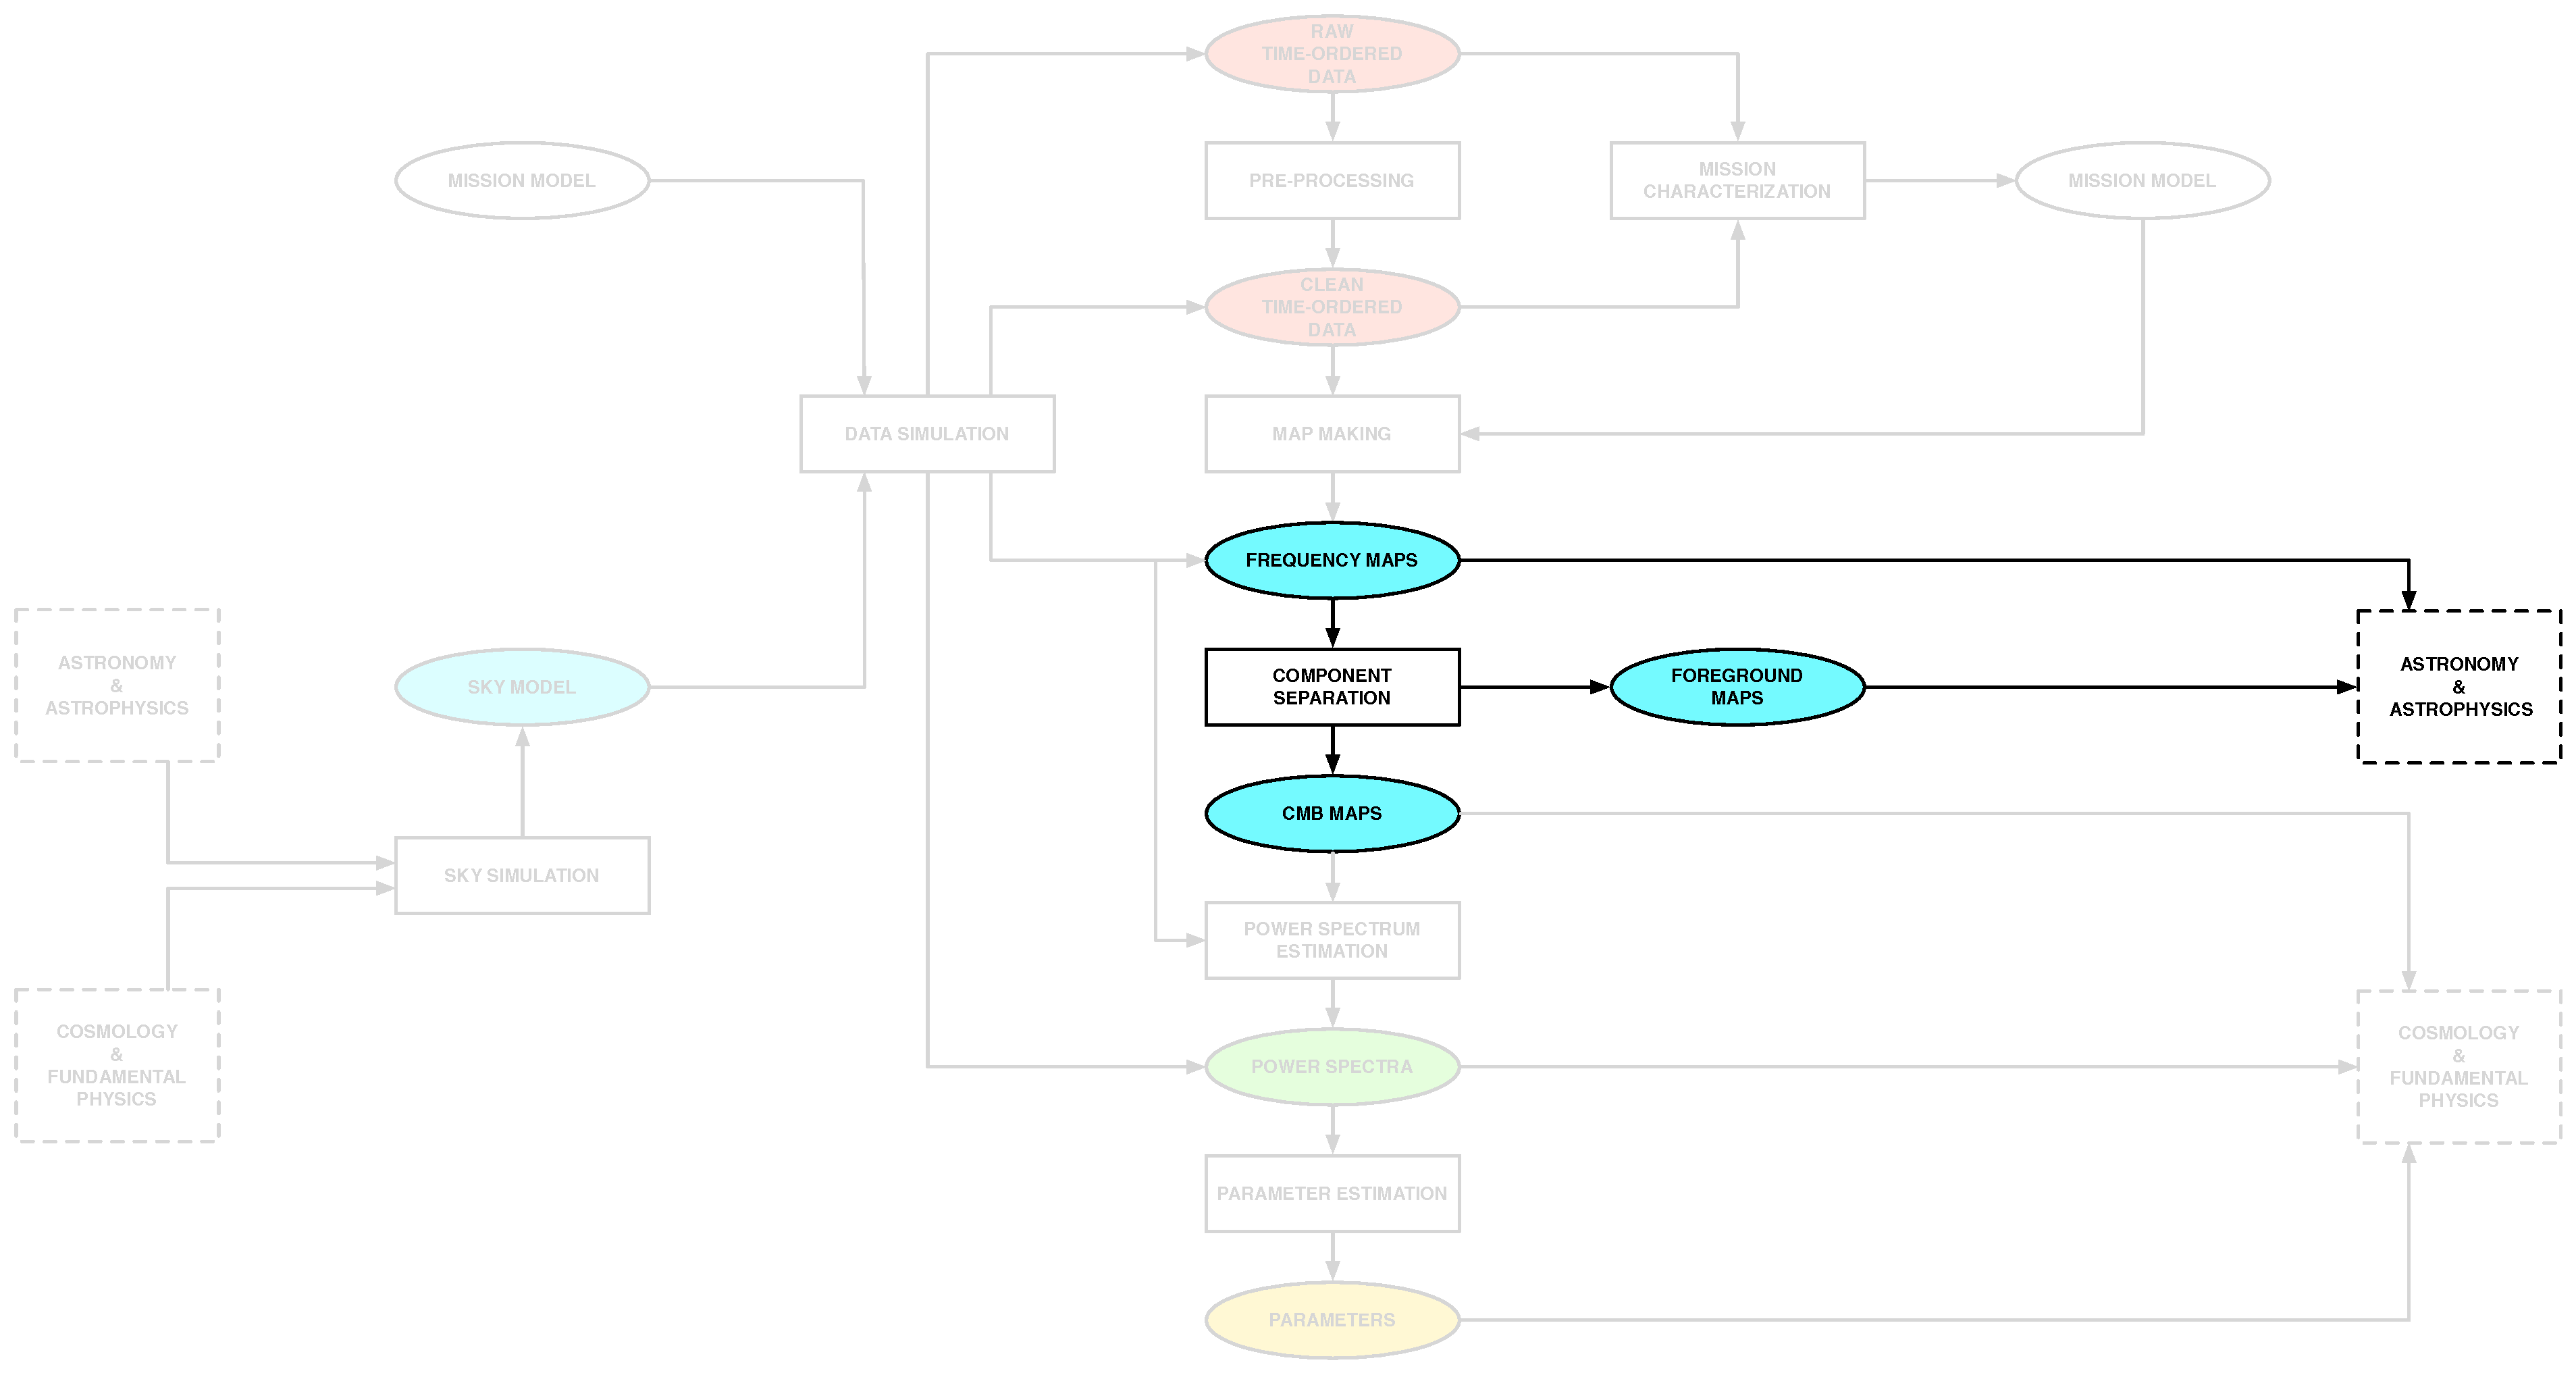
\includegraphics[width=1\textwidth]{Analysis/cs}
\caption{The component separation subset of the CMB simulation and data analysis pipeline}
\label{fig:general_comp_sep_scheme}
\end{figure*}

This section discusses the algorithms and methods disentangling sky emissions from multi-frequency maps. 
We first present the motivations and the general ideas of existing methods. 
We then give the specificities of parametric and blind methods. 
Finally, we summarize several questions which might be answered by follow-up studies.

\subsection{Introduction}

\begin{figure*}[htbp]
\centering
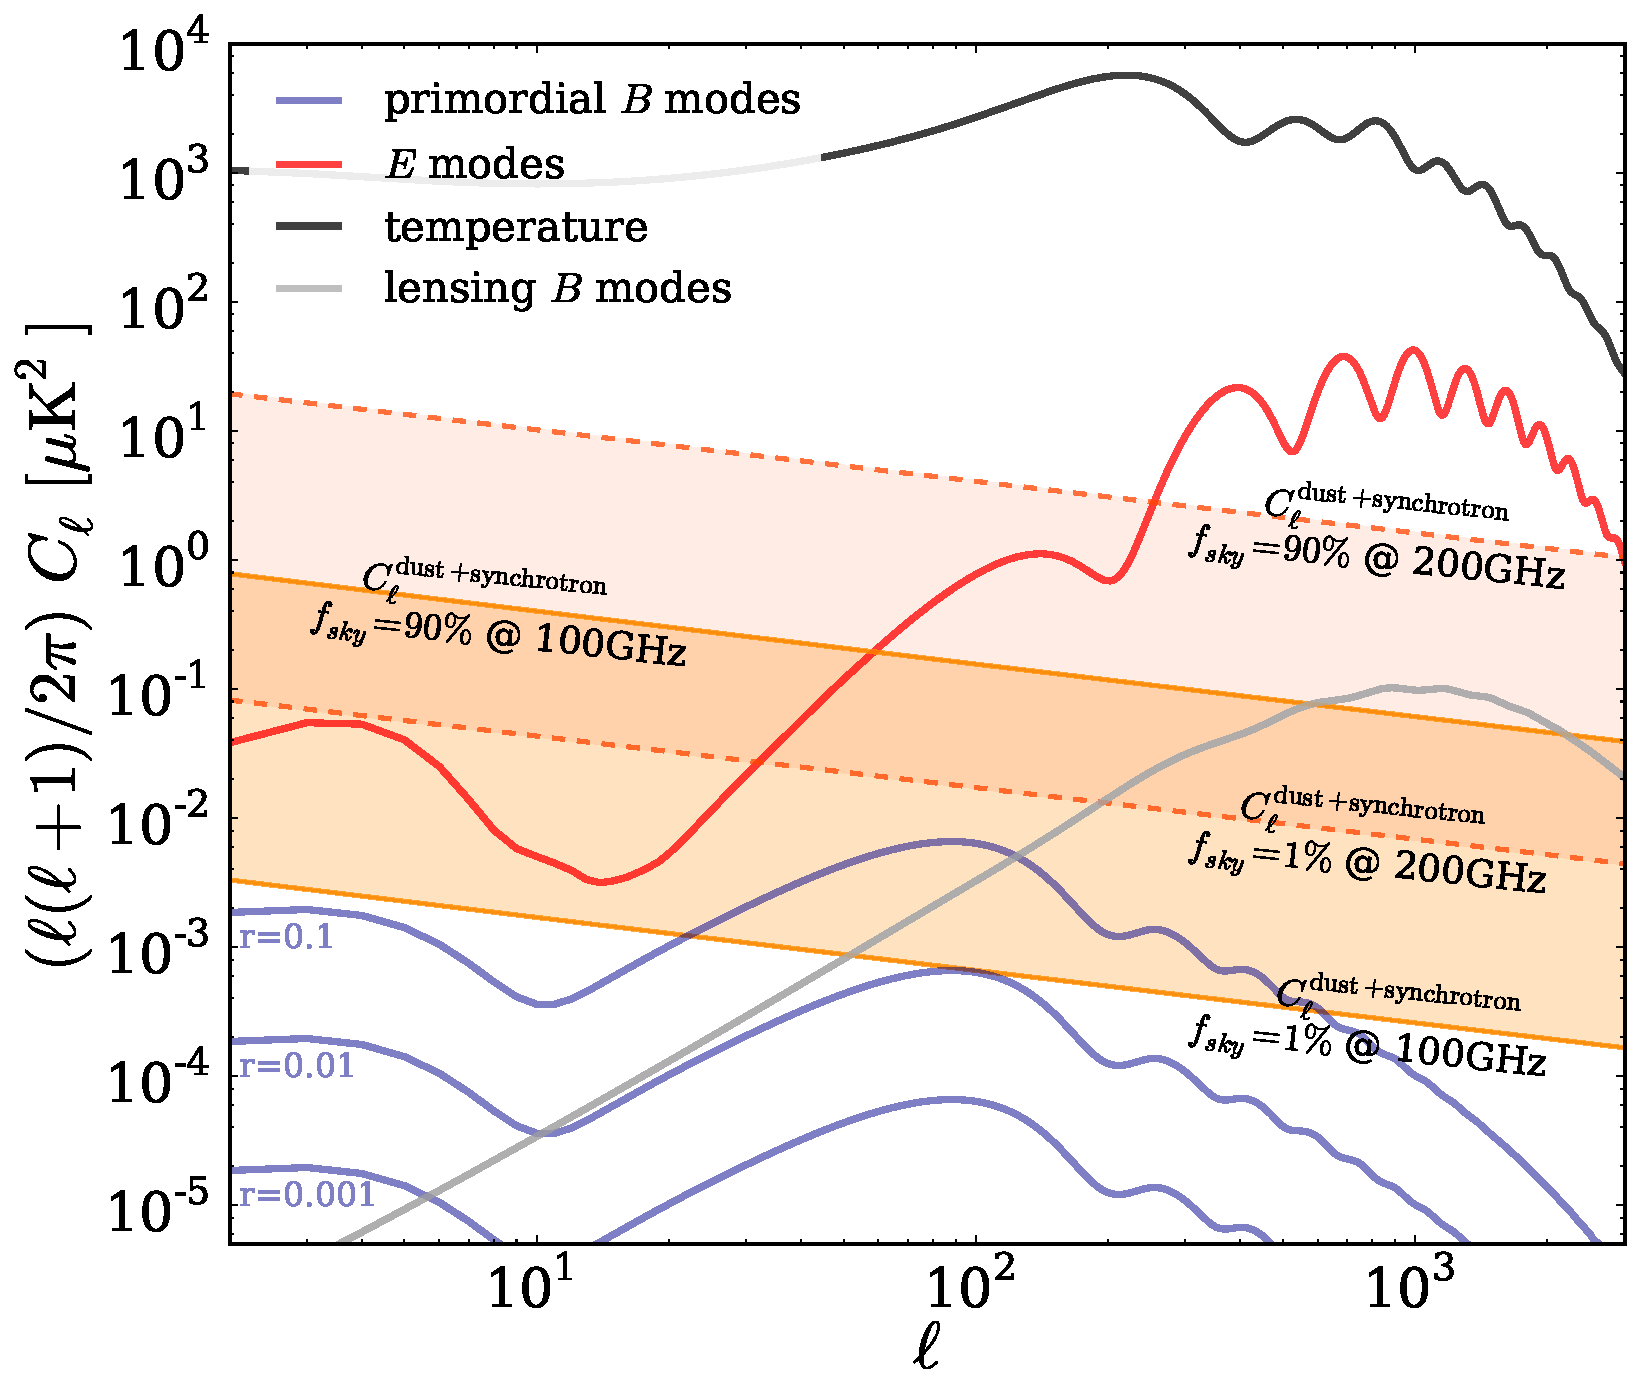
\includegraphics[width=0.5\textwidth]{Analysis/Power_Spectrum_figure_showing_foregrounds.pdf}
\caption{Angular power spectra showing primordial $B$ modes, lensing $B$ modes, total intensity, and $E$ modes, as well as the total contribution of polarized $B$-mode foregrounds (dust plus synchrotron), expected on the cleanest $1-90\%$ of the sky, at $100$ and $200\;$GHz. Note that, as these results are derived from Planck's Galactic masks and are not therefore optimized for high-resolution, ground-based instruments, there is potential for discovery of small patches of sky (e.g., $f_{\mathrm sky} \leq 5\%$) cleaner than those indicated here. From~\cite{}.}
\label{default}
\end{figure*}


\subsubsection{Motivations}

\textcolor{red}{JE: S4 science goals are $r$ and neutrino mass
\begin{itemize}
	\item component separation is obviously a necessary step to go beyond current constraints on e.g. primordial B-modes, cf. e.g. Fig.  of Errard et al (2015) --- foregrounds residuals coudl be expected to be dominant on largest scales?
	\item for neutrino mass, I suppose $C_\ell^{dd}$ has the best lever-arm, and we should evaluate the impact of foregrounds on the 4-point function (E-B estimators I suppose). NB: Planck lensing 2015 is based on SMICA map. Yet, the use of multiple-resolution maps degrades the final resolution of the component separated maps compared to a simple quadratic combination of beams weighted by their corresponding sensitivity. This might impact constraints on the lensing BB peak.
\end{itemize}}

%%%%%%%%%%%%%%%%%%%%%%
\subsubsection{Definition of component separation}
The general data modeling reads
\begin{eqnarray}
	\centering	
		d_p &=& \sum_{\rm comp, p} a_p^{\rm comp} s^{\rm comp}_p + n_p\\
		 &\equiv& \mathbf{A}\,s_p + n_p
	\label{eq:comp_sep_data_modeling}
\end{eqnarray}
where the vector $d_p$ contains the measured amplitude from each frequency map, $\mathbf{A}$ is the so-called mixing matrix which encapsulates the emission law $a_p^{\rm comp}$ of each component, $s_p$ is a vector containing the unknown CMB and foregrounds amplitude and $n_p$ is a vector containing the noise level for each frequency band. The index $p$ refers to sky pixels $\left( \theta, \phi \right)$, or modes of a spherical harmonic decomposition $\left( \ell, m\right)$, or a set of Fourier modes $\left(k_x,k_y\right)$, etc. Note that this modeling assumes spatial templates $s_p$ to be the same at all frequencies of observations.

Component separation aims at inverting Eq.~\ref{eq:comp_sep_data_modeling}, to estimate the foregrounds-distangled CMB signal encapsulated in $s_p$, as well as the foregrounds template which are relevant to test and update the sky modeling, cf. Fig.~\ref{fig:general_comp_sep_scheme}.
The estimate $\tilde{s}_p$ of the true sky templates $s_p$ --- given $\mathbf{A}$, $d_p$ and the statistical properties of the noise --- minimizes the following $\chi^2$:
\begin{eqnarray}
	\centering
		\chi^2 \equiv \sum_p \left| s_p - \tilde{s}_p\right|^2
	\label{eq:chi2_compsep}
\end{eqnarray}
and can be taken to have the following general form
\begin{eqnarray}
	\centering
		\tilde{s}_p = \mathbf{W}\,d_p
	\label{eq:sp_solution}
\end{eqnarray}
where the weighting operator $\mathbf{W}$ is chosen to optimize some criterion regarding $\tilde{s}_p$ and $s_p$ (variance of the cleaned map, unbiasedness, etc.) while keeping statistical consistency and robustness. In particular, a common requirement for all component separation algorithms is the ability of propagating errors due to foreground subtraction, while having the flexibility of including foreground modeling and external constraints in a transparent way. 
Component separation is a method consisting in estimating the mixing matrix $\mathbf{A}$ and eventually in finding the best $\mathbf{W}$ to get the closest possible estimate $\tilde{s}_p$ to the true sky signal.

For example, a solution to Eqs.~\ref{eq:chi2_compsep} and~\ref{eq:sp_solution} is obtained by taking $\mathbf{W} \equiv \left( \mathbf{A}^T\mathbf{N}^{-1}\mathbf{A} \right)^{-1}\mathbf{A}^T\mathbf{N}^{-1}$, leading to an unbiased estimate of the sky. As mentioned below, this expression can be changed, cf. e.g., Delabrouille \& Cardoso (2009), depending on the level of generality, complexity and prior knowledge on the sky signal analysts and observers want or are able to use. 


\textcolor{red}{JE: The component separation methods would generally
\begin{itemize}
	\item include any data processing that characterizes and exploit correlations between multi-frequencies observations,
	\item put external constraints and physical modeling
	\item and it would aim at distinguishing between different physical sources of emission.
	%NB For a given method, one would think that there should be a validation step (do the tools work on reasonable sky models?) and a verification step (are the sky models consistent with reality?). The second step is obviously the most difficult to answer.
\end{itemize}
$\rightarrow$ feedback from Planck component separation as well as the early CMB cleaning achieved in the BKP measurements + Stivoli et al (2010) + Fantaye et al (2011+2012) + Errard et al (2011+2012+2015).}

%%%%%%%%%%%%%%%%%%%%%%
\subsection{Description of methods}

We distinguish methods based on the internal template subtraction (e.g. Bennett et al. 1992; Hansen et al. 2006), those exploiting statistical independence of sky components (e.g. Delabrouille et al. 2003; Maino et al. 2007; Bonaldi et al. 2006), those invoking the maximum-entropy principle (e.g. Stolyarov et al. 2005), or performing a parametric fit to the data (Brandt et al. 1994; Eriksen et al. 2006).

\begin{itemize}
	\item \textbf{Parametric} -- The overall idea of these methods boils down to two steps: 1) the estimation of the mixing matrix, $\mathbf{A}$; and 2) the inversion of Eq.~\ref{eq:comp_sep_data_modeling} to recover an estimate of the sky signal, $s_p$.
	Parametric methods assumes that the mixing matrix, used in Eq.~\ref{eq:comp_sep_data_modeling}, has a functional form which is known and which can be parametrized by so-called "spectral" parameters $\beta$ i.e. $\mathbf{A} = \mathbf{A}(\beta)$. The functional form of $\mathbf{A}$ being fixed, the estimation of the mixing matrix is therefore equivalent to an estimation of the parameters $\beta$. The parameters of the model are determined via a fitting procedure, often performed on a pixel-by-pixel basis. This can be achieved by maximizing the following so-called "spectral" likelihood cf. Brandt et al (1994), Eriksen et al (2006):
	\begin{eqnarray}
		\centering
			-2\log \mathcal{L}(\beta) = - \sum_p \left( \mathbf{A}^T\mathbf{N}^{-1} d\right)^T\left( \mathbf{A}^T\mathbf{N}^{-1} \mathbf{A}\right)^{-1}\left( \mathbf{A}^T\mathbf{N}^{-1} d\right)
	\end{eqnarray}
Any deviation between the true mixing matrix $\mathbf{A}$ and the estimated $\mathbf{\tilde A} \equiv A(\tilde \beta)$ leads to the presence of foregrounds residuals in the reconstructed components maps.
	\textcolor{red}{JE: to be completed}\\
	\item \textbf{Blind} -- By assuming that sky components are statistically independent, blind methods aim at recovering these with an a priori unknown mixing matrix. Blind methods make minimal assumptions on the foregrounds and focus on the CMB reconstruction from its well known black body spectral energy distribution. The Internal Linear Combination (ILC, Tegmark et al. 2003) belongs to this class of methods. It only uses the CMB column of the mixing matrix elements (noted $a$ hereafter) to perform the minimum variance reconstruction, cf. Eq.~\ref{eq:sp_solution}:
\begin{equation}
  \tilde s_p = \sum_{i=0}^{i=m} w_i d_{p,i}
\end{equation}
with $\sum_i  w_i a_i = 1$, leading to the following solution:
\begin{equation}
  w_i = a^T N^{-1} (a^TN^{-1} a)^{-1}
\end{equation}

In this scheme, no attempt is made to design a foreground model. The decorrelation property between CMB and foregrounds alone is used to project out the contamination into a $m$-1 subspace (with $m$ being the number of frequency maps).

The main caveat in this method is its well known bias (Hinshaw 2007, Delabrouille 2009, etc) which comes from empirical correlation between the CMB and the foregrounds. The ILC bias is proportional to the number of detectors $m$ and inversely proportional to the number of pixels used to compute $N$. In order to reduce this effect, one could think of reducing the foreground subspace size by adding further constraints. The SEVEM template fitting method (Martinez-Gonzales et al 2003, etc) follows this idea, by building some foreground templates with a combination of a subset of the input frequency maps.

The semi-blind SMICA method (Cardoso et al 2008) also works at containing the foreground in a smaller dimension space, but in a more general way. The idea of Independent Component Analysis (ICA) is to blindly recover the full mixing matrix $\mathbf{A}$ by using the independence property of the different components. As we know that they are spatial correlations between the foregrounds, the ICA principle is used to disentangle the CMB from the noise and the foregrounds taken as a whole.

The main advantage of such blind of semi-blind methods is their ability to face any unknown and/or complex foreground contamination, to reconstruct a clean CMB signal. This is a big advantage when real data comes, one can then focus on instrumental effects, or data set combination issues at first, and leave the complex task of the foreground modeling and reconstruction for a future analysis step.

Moreover, in a framework like SMICA, the level of blindness can be adjusted via the plugin of any parametric component to its flexible engine as described in Cardoso et al 2008, allowing for a step by step fine grain design of the foreground model.\\
	\item \textbf{Discussion regarding the domain of application (harmonic, pixel, wavelet,etc.)} -- the implementation of Eq.~\ref{eq:sp_solution} can be implemented equivalently with any representations of the maps i.e. pixel, harmonic, wavelet, etc. The resulting separation is independent of this choice as long as the linear data modeling holds, Eq.~\ref{eq:comp_sep_data_modeling}. That said, the difference between domain of application will lie in the computational needs: for high number of sky pixels, the implementation of Eq.~\ref{eq:sp_solution} might be significantly more efficient in harmonic space.
\end{itemize}

\textcolor{red}{JE: $\rightarrow$ Parametric fitting vs. ILC, spatial domain versus non-spatial, that makes a basis of 4 algorithms. Although it was never quantified, the independence of those and very different hypotheses represent an opportunity for cross-checking and robustness.}

%%%%%%%%%%%%%%%%%%%%%%
\subsection{Questions to be addressed during follow-up studies}
\begin{itemize}
	\item \textbf{E/B or Q/U basis of analysis} -- \textcolor{red}{Maude ? Jonathan ?}
	\item \textbf{Multi-sites} -- \textcolor{red}{Carlo ? Jonathan ? }
	\item \textbf{Various resolutions} -- under the approximation that the mixing matrix is not significantly varying under the largest resolution, the impact of various resolutions can be propagated to the noise level of the final CMB map through the CMB x CMB term of $\left(\mathbf{A}^T\mathbf{N}^{-1}\mathbf{A}\right)^{-1}$ as given by Eq.~\ref{eq:sp_solution} with $\mathbf{W} \equiv \left( \mathbf{A}^T\mathbf{N}^{-1}\mathbf{A} \right)^{-1}\mathbf{A}^T\mathbf{N}^{-1}$. Beam for each frequency channel would appear in the expression of the noise covariance matrix 
	\begin{eqnarray}
		\centering
			\mathbf{N}(i) \equiv \mathbf{N}(i)_\ell = \sigma(i)^2\exp\left[ \frac{\ell(\ell+1)\theta_{\rm FWHM}^2}{8\log(2)} \right]
	\end{eqnarray}
	where $i$ is a frequency channel. The noise variance after component separation would then be given by
	\begin{eqnarray}
		\centering
			N_\ell^{\rm post\ comp\ sep} = \left[\left(\mathbf{A}^T\left(\mathbf{N}_\ell\right)^{-1}\mathbf{A}\right)^{-1}\right]_{\rm CMBxCMB}
	\end{eqnarray}
	\item \textbf{Atmosphere residuals} -- Atmosphere residuals appear on large scale in CMB observations, and they scale with frequency in a similar way as dust, cf. Errard et al (2015a). Having redundant frequencies among the different observatories could help mitigating the atmospheric and astrophysical foregrounds.
\end{itemize}

\textcolor{red}{JE: we could outline a roadmap, i.e. the application and learning phase to SIV made by the various sub-orbitals which are going on-line now or soon with the usual 95, 150, 220. That would need to be investigated very accurately as it would represent a most important step for component separation towards SIV.}



%\bibliography{cmbs4}

%%
%% Populate the .bib file with entries from SPIRES Bibtex (preferred)
%% or ADS Bibtex (if no SPIRES entry).
%%  SPIRES will also supply the CITATION line information; please include it.
%%


